
%(BEGIN_QUESTION)
% Copyright 2007, Tony R. Kuphaldt, released under the Creative Commons Attribution License (v 1.0)
% This means you may do almost anything with this work of mine, so long as you give me proper credit

A level indicator is registering a liquid level that is falsely high.  The operator has hand-gauged the storage vessel with a tape measure and determined the actual level to be 8.2 feet, but the level indicator (LI) registers 10.1 feet.  The calibrated range of the 3-15 PSI pneumatic transmitter is 0 feet to 12 feet.  You measure the pneumatic pressure signal with a test gauge and find that it is 13.1 PSI.  Which instrument is at fault in this system?  How do you know?

$$\includegraphics[width=15.5cm]{i02961x01.eps}$$

Furthermore, identify whether the fault is a {\it zero shift}, a {\it span shift}, a problem with {\it linearity}, {\it hysteresis}, or whether it is impossible to determine from the information we have.

\vfil 

\underbar{file i02961}
\eject
%(END_QUESTION)





%(BEGIN_ANSWER)

This is a graded question -- no answers or hints given!

%(END_ANSWER)





%(BEGIN_NOTES)

An important principle to apply when isolating calibration errors and other instrument loop faults is that {\it every instrument has at least one input and one output, and the signals at each of these should correlate with each other}.  Whichever instrument in a loop fails this correlation test is the one to blame.

\vskip 10pt

In this example, we may compare the known liquid level to the transmitter's output signal to see if those two values properly correlate.  If so, the transmitter is functioning properly; if not, the transmitter is at fault.  Likewise, we may compare the pneumatic signal to the indicator's reading to see if those two values properly correlate.  If so, the indicator is functioning properly; if not, the indicator is at fault.

\vskip 10pt

The measured pneumatic pressure signal of 13.1 PSI correlates to a percentage value of 84.17\%.  This agrees with the indicator's reading of 10.1 feet (in a 0-12 foot range), but it does not agree with the actual process liquid level of 8.2 feet.

\vskip 10pt

Therefore, the indicator cannot be at fault.  The only possible faults remaining are the {\bf transmitter} and the operator's {\bf hand gauge}.  Of those two, it is more likely that the transmitter has some sort of problem than a human operator missed the mark by almost two feet!  The specific nature of this fault is impossible to tell, as we have only one point of data.  If we had multiple points of data, we could better identify what type of mis-calibration error this is (e.g. zero shift versus span shift versus linearity versus hysteresis).

%INDEX% Calibration errors, identifying the location of in a loop
%INDEX% Measurement, level: troubleshooting

%(END_NOTES)


